% ---
% Capitulo de Resultados
% ---

\chapter{Resultados\label{cha:results}}

Este capítulo apresenta os resultados, organizados na ordem das questões de pesquisa do Capítulo \ref{cha:intro}. As Seções \ref{sec:res-bridges} e \ref{sec:res-connectivity} tratam da QP3, isto é, da substituição da árvore geradora por uma estimativa. A Seção \ref{sec:res-memory} responde à QP1 sobre a memória por dispositivo, e a Seção \ref{sec:res-scale} verifica que a resposta se sustenta em escala. A Seção \ref{sec:res-overlap} responde à QP2 sobre o custo do particionamento em qualidade e sobre o parâmetro que o controla. As Seções \ref{sec:res-scaling} a \ref{sec:res-extract} respondem à QP4 sobre o custo em tempo e sobre o que a decomposição oferece em contrapartida. A Seção \ref{sec:res-parity} verifica que nenhuma afirmação depende do ambiente de execução, e a Seção \ref{sec:res-sensitivity} caracteriza a sensibilidade aos parâmetros livres.

% =====================================================================
\section{Procedência das medições\label{sec:res-provenance}}
% =====================================================================

Todos os números apresentados neste capítulo provêm de medições do método como descrito no Capítulo \ref{cha:methods}, tomadas no agregado de quatro \ac{GPU}s descrito na Seção \ref{sec:hardware}, sobre até 5 sementes aleatórias, sem execuções falhas. A política de sementes é a da Seção \ref{sec:hardware}: múltiplas sementes onde o NN-Descent intervém, duas onde o \ac{k-NNG} é mantido exato e a execução é determinística.\\

Duas medições precedem o conjunto atual e são reportadas sem reexecução, porque a grandeza que cada uma reporta não é afetada pelo trabalho de implementação realizado desde então: a Tabela \ref{tab:bridges}, que mantém a metade de vizinhança exata nos dois braços, e a Figura \ref{fig:components}, que conta componentes.\\

% =====================================================================
\section{As pontes anti-hub reproduzem a árvore geradora exata\label{sec:res-bridges}}
% =====================================================================

Pontes só podem ser avaliadas onde o \ac{k-NNG} de fato se fragmenta. A Tabela \ref{tab:bridges} restringe-se aos conjuntos de dados em que isso ocorre, com o \ac{k-NNG} mantido exato nos dois lados da comparação, de modo que a estimativa de pontes seja a única variável. Como a referência é uma árvore geradora de custo $O(n^2 d)$, toda linha executa em $n = 4.000$; o conjunto \texttt{sift1m} aparece aqui, portanto, com dois componentes, ao passo que em seu $n$ completo o mesmo conjunto é conexo, conforme a Tabela \ref{tab:datasets}.\\

\begin{table}[htb!]
\caption{\label{tab:bridges} Pontes anti-hub contra a $\mathrm{MST}_{\kmax}$ exata, com $n = 4.000$ em toda linha. Ambos os lados compartilham um \ac{k-NNG} exato. A aceleração é a da construção das pontes contra a árvore geradora exata que elas substituem.}
\centering
\footnotesize
\begin{tabular}{@{}lrrrr@{}}
\toprule
conjunto de dados & comp. & razão de peso & ARI & aceleração \\
\midrule
\texttt{manifold\_c32}  & 32 & 1,00022 & 1,0000 & 18,2$\times$ \\
\texttt{manifold\_c24}  & 24 & 1,00024 & 1,0000 & 36,0$\times$ \\
\texttt{manifold\_exact}& 16 & 1,00000 & 1,0000 & 12,1$\times$ \\
\texttt{manifold\_c8}   & 8  & 1,00001 & 1,0000 & 19,0$\times$ \\
\texttt{sift1m}         & 2  & 1,00000 & 1,0000 & 10,5$\times$ \\
\bottomrule
\end{tabular}\\
Fonte: Autoral.
\end{table}

O pior caso observado em qualquer configuração é uma árvore geradora 0,024\% mais pesada que a ótima, com \ac{ARI} do DBSCAN* exatamente 1,0000, por 10,5 a 36 vezes menos trabalho. A razão de peso é uma afirmação sobre as alturas de fusão do dendrograma, de modo que o \ac{ARI} unitário é a consequência esperada: a estimativa produz árvores cuja sequência de fusões é indistinguível da exata nos limiares que importam para a extração de grupos. O mesmo efeito é observável fora da escala em que a referência exata é viável, e a medição correspondente está na Seção \ref{sec:res-sensitivity}: em $n = 50.000$, o \ac{k-NNG} de \texttt{manifold\_wide} se divide em 300 componentes e as pontes o reduzem a exatamente um, em todas as sementes. Essa contagem usa a grandeza corrigida descrita na Seção \ref{sec:metrics}; a versão inicial era registrada depois de as pontes serem incorporadas à rotulação, e por isso lia 1 por construção.\\

A razão de peso é a coluna que sustenta essa afirmação, e a coluna de \ac{ARI} deve ser lida com uma ressalva, estabelecida durante a ablação da Seção \ref{sec:res-connectivity}. O limiar em que ambas as árvores são cortadas é o peso médio das arestas da árvore exata, que fica bem abaixo das alturas de fusão que uma ponte afeta, e os dois braços desta tabela compartilham todas as arestas do \ac{k-NNG} por construção. As duas rotulações concordam, portanto, sobre as arestas curtas, independentemente do que as pontes fizeram, e um valor de 1,0000 reflete em parte essa insensibilidade, além da qualidade da estimativa. A razão de peso e a diferença pontual entre os perfis comparam as árvores diretamente e não compartilham essa limitação.\\

A quantidade de anti-hubs selecionados influencia essa qualidade, mas de forma dependente do conjunto de dados. A Tabela \ref{tab:antihub-count} apresenta a varredura sobre o conjunto \texttt{manifold\_c24}, com o \ac{k-NNG} mantido exato. A melhora é monótona e substancial nesse caso.\\

\begin{table}[htb!]
\caption{\label{tab:antihub-count} Razão de peso da árvore geradora em função da quantidade de anti-hubs selecionados, \texttt{manifold\_c24} (24 componentes), \ac{k-NNG} mantido exato nos dois lados.}
\centering
\footnotesize
\begin{tabular}{@{}lrrrrr@{}}
\toprule
anti-hubs & 4 & 16 & 64 & 256 & 1024 \\
\midrule
razão de peso & 1,01213 & 1,01206 & 1,00813 & 1,00167 & 1,00016 \\
\bottomrule
\end{tabular}\\
Fonte: Autoral.
\end{table}

Esse comportamento, contudo, não generaliza, e a advertência é parte do resultado. Em conjuntos de baixa dimensionalidade com grupos aproximadamente esféricos a mesma varredura é plana, com 4 anti-hubs produzindo praticamente o mesmo resultado que 1024, o que indica sobreprovisionamento. Em dados reais cujo \ac{k-NNG} é conexo a varredura é irrelevante, pois não há nada a conectar. A sensibilidade à quantidade de anti-hubs é, portanto, uma propriedade da estrutura de componentes dos dados, antes que do método. O custo é aproximadamente constante até cerca de 256 anti-hubs, o que sustenta dimensionar o conjunto por uma medida de dimensionalidade acompanhada de um multiplicador, em lugar de uma contagem absoluta fixa.\\

Um erro de medição encontrado durante esses experimentos produziu uma tabela incorreta antes de ser identificado. Comparar dois objetos \ac{CORE-SG} construídos separadamente não isola o efeito das pontes: cada um recebe seu próprio \ac{k-NNG} aleatorizado, e o ruído dessa diferença excede o sinal buscado, manifestando-se como uma razão de peso abaixo de 1,0, o que é impossível para uma aproximação genuína. Toda comparação de qualidade de pontes precisa forçar os dois lados a compartilhar um \ac{k-NNG} exato e idêntico.\\

% =====================================================================
\section{Grafos de vizinhança reais já são conexos\label{sec:res-connectivity}}
% =====================================================================

A Figura \ref{fig:components} reporta a contagem de componentes do \ac{k-NNG} sozinho em função de $\kmax$, e a Tabela \ref{tab:connectivity} apresenta os valores dos conjuntos reais, onde a diferença entre um e dois componentes não é legível em escala logarítmica. Todo conjunto de dados real examinado se torna conexo em $\kmax \leq 24$, e a faixa de operação deste trabalho e do trabalho original do \ac{CORE-SG} \cite{core-sg} é de 24 a 32. Os conjuntos sintéticos da família \textit{manifold} não se tornam conexos em nenhum $\kmax$ da faixa, o que é precisamente a razão de sua existência.\\

\begin{figure}[htb!]
\centering
\caption{\label{fig:components} Componentes do \ac{k-NNG} sozinho, em $n$ completo, média de 3 sementes. Todo conjunto de dados real alcança um único componente em $\kmax \leq 24$; os conjuntos sintéticos nunca o fazem. A dimensionalidade ambiente não explica o limiar: \texttt{20ng\_tfidf} ($d=1000$) conecta em $\kmax = 4$ enquanto \texttt{gist1m} ($d=960$) exige $\kmax = 24$.}
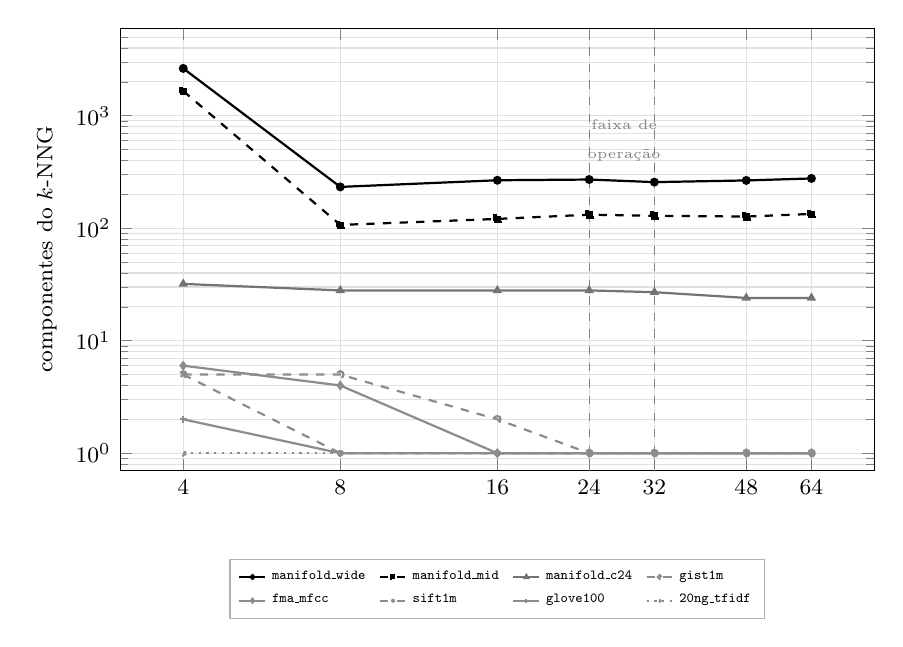
\begin{tikzpicture}
\begin{axis}[
  width=0.92\textwidth, height=7.2cm,
  xlabel={$\kmax$}, ylabel={componentes do $k$-NNG},
  ymode=log, log basis y=10,
  xmode=log, log basis x=2, xtick={4,8,16,24,32,48,64},
  xticklabels={4,8,16,24,32,48,64},
  ymin=0.7, ymax=6000,
  grid=both, grid style={black!12},
  legend style={font=\tiny, at={(0.5,-0.20)}, anchor=north,
                legend columns=4, draw=black!30, legend cell align=left,
                /tikz/every even column/.append style={column sep=1mm}},
  legend image post style={scale=0.55},
  label style={font=\footnotesize}, tick label style={font=\footnotesize},
  every axis plot/.append style={thick, mark size=1.2pt}
]
\addplot[mark=*, black] coordinates {(4,2636)(8,233)(16,267)(24,271)(32,257)(48,266)(64,277)};
\addlegendentry{\texttt{manifold\_wide}}
\addplot[mark=square*, black, dashed] coordinates {(4,1658)(8,107)(16,121)(24,132)(32,129)(48,127)(64,134)};
\addlegendentry{\texttt{manifold\_mid}}
\addplot[mark=triangle*, black!55] coordinates {(4,32)(8,28)(16,28)(24,28)(32,27)(48,24)(64,24)};
\addlegendentry{\texttt{manifold\_c24}}
\addplot[mark=o, black!45, dashed] coordinates {(4,5)(8,5)(16,2)(24,1)(32,1)(48,1)(64,1)};
\addlegendentry{\texttt{gist1m}}
\addplot[mark=diamond*, black!45] coordinates {(4,6)(8,4)(16,1)(24,1)(32,1)(48,1)(64,1)};
\addlegendentry{\texttt{fma\_mfcc}}
\addplot[mark=x, black!45, dashed] coordinates {(4,5)(8,1)(16,1)(24,1)(32,1)(48,1)(64,1)};
\addlegendentry{\texttt{sift1m}}
\addplot[mark=+, black!45] coordinates {(4,2)(8,1)(16,1)(24,1)(32,1)(48,1)(64,1)};
\addlegendentry{\texttt{glove100}}
\addplot[mark=asterisk, black!45, dotted] coordinates {(4,1)(8,1)(16,1)(24,1)(32,1)(48,1)(64,1)};
\addlegendentry{\texttt{20ng\_tfidf}}
\draw[gray, dashed] (axis cs:24,0.7) -- (axis cs:24,6000);
\draw[gray, dashed] (axis cs:32,0.7) -- (axis cs:32,6000);
\node[font=\tiny, gray, anchor=south] at (axis cs:28,620) {faixa de};
\node[font=\tiny, gray, anchor=north] at (axis cs:28,620) {operação};
\end{axis}
\end{tikzpicture}\\
Fonte: Autoral.
\end{figure}

\begin{table}[htb!]
\caption{\label{tab:connectivity} Componentes do \ac{k-NNG} sozinho, em $n$ completo, grafo aproximado, média de 3 sementes. Em negrito, o menor $\kmax$ em que o conjunto se torna conexo.}
\centering
\footnotesize
\begin{tabular}{@{}lrrrrrrr@{}}
\toprule
conjunto de dados & $k=4$ & $k=8$ & $k=16$ & $k=24$ & $k=32$ & $k=48$ & $k=64$ \\
\midrule
\texttt{20ng\_pca500} & \textbf{1} & 1 & 1 & 1 & 1 & 1 & 1 \\
\texttt{20ng\_tfidf}  & \textbf{1} & 1 & 1 & 1 & 1 & 1 & 1 \\
\texttt{glove100}     & 2 & \textbf{1} & 1 & 1 & 1 & 1 & 1 \\
\texttt{sift1m}       & 5 & \textbf{1} & 1 & 1 & 1 & 1 & 1 \\
\texttt{fma\_chroma}  & 8 & 2 & \textbf{1} & 1 & 1 & 1 & 1 \\
\texttt{fma\_mfcc}    & 6 & 4 & \textbf{1} & 1 & 1 & 1 & 1 \\
\texttt{gist1m}       & 5 & 5 & 2 & \textbf{1} & 1 & 1 & 1 \\
\midrule
\texttt{manifold\_mid}  & 1658 & 107 & 121 & 132 & 129 & 127 & 134 \\
\texttt{manifold\_wide} & 2636 & 233 & 267 & 271 & 257 & 266 & 277 \\
\bottomrule
\end{tabular}\\
Fonte: Autoral.
\end{table}

Três observações decorrem desses dados.\\

A primeira observação é que a árvore geradora corrige a fragmentação do grafo de vizinhança e contribui pouco além disso em dados conexos. Onde o \ac{k-NNG} já é um único componente, as pontes não têm o que ligar, do que se poderia concluir que elas não alteram nada. A conectividade sozinha não estabelece isso, e \citeonline{core-sg} já o apontam em termos teóricos: um \ac{k-NNG} conexo pode não conter uma $\mathrm{MST}_{\mpts}$, e os autores exibem um contraexemplo em $k = \mpts = 4$. O que eles estabelecem é a possibilidade; o que esta seção acrescenta é a magnitude. Esse contraexemplo é a configuração em ferradura da Figura \ref{fig:coresg-edge-case}, descrita na Seção \ref{sec:coresg-why}: uma \ac{MST} sobre o grafo completo pode conter uma aresta curta ligando diretamente duas regiões que o \ac{k-NNG} só liga por um desvio longo em torno delas, de modo que os dois grafos são conexos e ainda assim induzem hierarquias diferentes. A Tabela \ref{tab:ablation} resolve a questão diretamente, extraindo uma árvore do \ac{k-NNG} sozinho, sem nenhuma ponte e sem reparo, e pontuando-a contra o \ac{CORE-SG} exato.\\

\begin{table}[htb!]
\caption{\label{tab:ablation} O \ac{k-NNG} sozinho contra o \ac{CORE-SG} exato, com o \ac{k-NNG} mantido exato nos dois lados. A coluna ``divergem'' conta as arestas da árvore exata que este braço não contém, entre as $n-1$ de uma árvore geradora. A razão de peso nunca pode cair abaixo de 1 para uma árvore geradora sobre um subgrafo, de modo que qualquer excesso é um desvio que as arestas do \ac{k-NNG} obrigaram. Duas sementes; $\kmax = 32$ em todas as linhas.}
\centering
\footnotesize
\begin{tabular}{@{}lrrrrrr@{}}
\toprule
 & & \multicolumn{3}{c}{divergem em $\mpts$} & \multicolumn{2}{c}{em $\mpts = \kmax$} \\
\cmidrule(lr){3-5}\cmidrule(lr){6-7}
conjunto de dados & $n$ & $\le 8$ & 16 & 32 & razão de peso & excesso \\
\midrule
\texttt{sift1m}    & 25 mil  & 0 & 1 & 1  & 1,0000027 & 2,7 ppm \\
                   & 50 mil  & 0 & 0 & 4  & 1,0000010 & 1,0 ppm \\
                   & 100 mil & 0 & 0 & 5  & 1,0000008 & 0,8 ppm \\
\texttt{fma\_mfcc} & 25 mil  & 0 & 0 & 8  & 1,0000012 & 1,2 ppm \\
                   & 50 mil  & 0 & 0 & 5  & 1,0000003 & 0,3 ppm \\
                   & 100 mil & 1 & 1 & 9  & 1,0000018 & 1,8 ppm \\
\texttt{glove100}  & 25 mil  & 0 & 2 & 5  & 1,0000043 & 4,3 ppm \\
                   & 50 mil  & 0 & 1 & 6  & 1,0000035 & 3,5 ppm \\
                   & 100 mil & 1 & 4 & 22 & 1,0000052 & 5,2 ppm \\
\midrule
\texttt{gist1m}    & 25 mil  & 0 & 0 & 0  & 1,0000000 & 0 \\
                   & 50 mil  & 0 & 0 & 0  & 1,0000000 & 0 \\
\bottomrule
\end{tabular}\\
Fonte: Autoral.
\end{table}

Da tabela decorrem três constatações, e a primeira é que a forma forte da afirmação é falsa. A razão de peso excede 1 em nove das onze configurações, e como ela não pode cair abaixo de 1 para uma árvore geradora sobre um subgrafo, isso significa que o \ac{k-NNG} sozinho força um desvio em algum lugar. Nas duas configurações restantes, ambas em \texttt{gist1m}, as duas árvores são idênticas aresta a aresta, e a razão é exatamente 1.\\

O efeito é também pequeno e confinado. Em $\mpts \leq 8$ as duas árvores são idênticas em nove das onze configurações, com uma única aresta divergente nas outras duas. Em $\mpts = 16$ elas permanecem idênticas em seis configurações e divergem em 1 a 4 arestas nas cinco restantes. As diferenças se concentram em $\mpts = \kmax$, onde alcançam de 0 a 22 arestas entre 25.000 e 100.000, e de 0,3 a 5,2 partes por milhão do peso total da árvore. Em \texttt{sift1m} com $n = 25.000$, a discrepância inteira é uma única aresta substituída, 18,85 mais pesada que a que ela substituiu, contra uma altura média de fusão de 281,8.\\

A concentração em valores grandes de $\mpts$ é o que a definição prevê. Em $\mpts$ pequeno as \textit{core distances} de \eqref{eq:mrd} são pequenas, de modo que a \textit{mutual reachability distance} é aproximadamente a distância métrica, as arestas mais baratas são as mais curtas, e essas são exatamente as que um \ac{k-NNG} armazena. Em $\mpts = \kmax$ as \textit{core distances} estão em seu maior valor, e todo ponto a distância menor que $\coredist^{\kmax}(x)$ de $x$ é um parceiro igualmente barato, ao mesmo peso; mas a fronteira dessa bola é justamente o $\kmax$-ésimo vizinho armazenado, de modo que parceiros empatados naquela distância são igualmente baratos e não couberam na lista. O conjunto \texttt{glove100} exibe o efeito com maior intensidade e é também o de maior dimensionalidade intrínseca entre os avaliados, onde tais empates são mais numerosos. Essa é a leitura que o padrão sustenta, e permanece uma conjectura: as arestas divergentes não foram inspecionadas individualmente.\\

A consequência prática é a mesma que motivou o projeto. As pontes rendem em uma faixa estreita próxima a $\mpts = \kmax$, e os agrupamentos planos cortados das duas árvores foram idênticos em todos os limiares aplicados. Derivar a rotulação de componentes custa de 0,08 a 3,5\,ms nos conjuntos avaliados, contra 5,3 a 222\,ms de trabalho de \textit{hubness} e de pontes, um fator de 48 a 136, de modo que testar a conectividade primeiro e pular o cálculo das pontes onde o grafo já é conexo custa pouco e abre mão de pouco.\\

Onde o grafo de fato se fragmenta, o quadro é inteiramente diferente, e é esse o controle de que a ablação precisa. Em \texttt{manifold\_mid} o \ac{k-NNG} sozinho deixa 150 componentes em todos os tamanhos testados, de modo que a estrutura extraída dele é uma floresta com 149 arestas a menos do que uma árvore geradora exigiria, e sua razão de peso, de 0,92 a 0,97, fica abaixo de 1 apenas porque é uma soma sobre menos arestas. Ali as pontes deixam de ser uma correção marginal e passam a ser o mecanismo que produz a árvore.\\

A segunda é que a dimensionalidade ambiente não prediz o limiar, como mostra o par de conjuntos destacado na legenda da Figura \ref{fig:components}. O que distingue os dois casos é a presença de componentes genuinamente separados por densidade, cada um contendo muitos pontos, propriedade que a família sintética possui por construção e que os dados reais, nessas escalas, majoritariamente não possuem.\\

A terceira é que a conectividade observada não vem da aproximação. Ela poderia ser um erro residual do NN-Descent, na forma de arestas longas entre componentes que conectassem um grafo que o \ac{k-NNG} exato deixaria em pedaços, e a medição afasta essa leitura. Na faixa de operação, o conjunto \texttt{manifold\_c24} produz 24 componentes com o grafo exato e de 25 a 29 com o aproximado, já que um vizinho não encontrado remove uma aresta enquanto um vizinho substituído permanece local. O efeito se inverte quando $\kmax$ se aproxima do tamanho do componente, caso de \texttt{manifold\_c32} em $\kmax = 64$, com 30 componentes no grafo aproximado contra 32 no exato, e por isso a afirmação é enunciada de forma restrita.\\

% =====================================================================
% =====================================================================
\section{Memória por dispositivo contra quantidade de instâncias\label{sec:res-memory}}
% =====================================================================

Esta seção responde à QP1. A Tabela \ref{tab:memory} reporta uma construção de $5 \times 10^5$ pontos em contagens de instâncias de 1 a 64, medida em quatro \ac{GPU}s com a sobreposição padrão $\omega = 1{,}0$. A grandeza reportada é a maior instância que um dispositivo precisou manter, que é o que decide se uma configuração cabe.\\

\begin{table}[htb!]
\caption{\label{tab:memory} Uma construção de \texttt{sift1m} e \texttt{glove100} em $n = 5 \times 10^5$, $\kmax = 32$, $\omega = 1{,}0$, em quatro \ac{GPU}s. A coluna \textit{residente} é a maior instância que um dispositivo precisou manter, e \textit{fator} é sua redução contra $m = 1$. A revocação é amostrada sobre 2.000 consultas pontuadas exatamente contra todos os pontos. Em negrito, o extremo de cada coluna: a maior revocação de cada conjunto, o maior fator de redução e a menor residência.}
\centering
\footnotesize
\begin{tabular}{@{}lrrrrr@{}}
\toprule
 & & \multicolumn{2}{c}{\texttt{sift1m}} & \multicolumn{2}{c}{\texttt{glove100}} \\
\cmidrule(lr){3-4}\cmidrule(lr){5-6}
instâncias & fator & residente & revocação & residente & revocação \\
\midrule
1  & 1,0$\times$  & 472,0\,MB & 0,9677 & 424,0\,MB & 0,7188 \\
2  & 1,4$\times$  & 329,1\,MB & \textbf{0,9814} & 295,6\,MB & 0,7799 \\
4  & 2,4$\times$  & 196,5\,MB & 0,9785 & 176,5\,MB & \textbf{0,7890} \\
8  & 4,4$\times$  & 107,7\,MB & 0,9741 & 96,7\,MB  & 0,7773 \\
16 & 8,4$\times$  & 56,4\,MB  & 0,9702 & 50,7\,MB  & 0,7646 \\
32 & 16,3$\times$ & 28,9\,MB  & 0,9669 & 25,9\,MB  & 0,7476 \\
64 & \textbf{32,3}$\times$ & \textbf{14,6\,MB} & 0,9645 & \textbf{13,1\,MB} & 0,7289 \\
\bottomrule
\end{tabular}\\
Fonte: Autoral.
\end{table}

A residência segue a Equação \eqref{eq:instancesize}: 472,0\,MB em uma instância e 14,6\,MB em 64, um fator de 32,3. O fator é 32 e não 64 porque $\omega = 1{,}0$ dobra o tamanho de cada instância, deixando $m = 1$ inalterado, caso em que os sorteios de sobreposição recaem sobre o próprio bloco único. Em $\omega = 0{,}05$ a mesma faixa produz 472,0\,MB contra 7,7\,MB, um fator de 61,0. As razões se mantêm em \texttt{glove100} e em toda contagem de dispositivos medida, já que a residência é determinada pela quantidade de instâncias e não por quantos dispositivos as executam.\\

A revocação não cai monotonicamente. Ela sobe de $m = 1$ para $m = 2$ nos dois conjuntos, em 0,0137 em \texttt{sift1m} e 0,0611 em \texttt{glove100}, atinge máximo em $m = 2$ no primeiro e em $m = 4$ no segundo, e declina a partir daí. Em $m = 1$ nenhum passo de reparo é executado. Em \texttt{glove100} toda contagem de 2 a 64 permanece acima do valor de $m = 1$, em 0,0702 no máximo e 0,0101 em $m = 64$; em \texttt{sift1m} as contagens de 2 a 16 permanecem acima, e $m = 32$ e $m = 64$ ficam 0,0008 e 0,0032 abaixo.\\

Esse comportamento contraria a expectativa. Particionar um conjunto de dados para construir um grafo de vizinhança deveria, pelo argumento da Seção \ref{sec:problem-partition-cost}, apenas piorar o resultado. O que a tabela mostra é que o passo de reparo, operando sobre um grafo mesclado que já possui vizinhanças razoáveis, encontra arestas que uma descida única partindo de um grafo aleatório não encontra dentro do mesmo orçamento de rodadas. A decomposição, portanto, não troca apenas qualidade por memória: em contagens baixas de instâncias ela melhora as duas.\\

O custo em tempo de relógio da mesma faixa é de 5,862\,s em $m = 1$ contra 10,033\,s em $m = 64$ em \texttt{sift1m}, um fator de 1,71. Em uma única \ac{GPU} a mesma comparação é de 5,757\,s contra 15,774\,s, um fator de 2,74; a Seção \ref{sec:res-overlap} separa as duas.\\

% =====================================================================
\section{Sobreposição de instâncias\label{sec:res-overlap}}
% =====================================================================

Esta seção responde à QP2. A fração de sobreposição $\omega$ da Equação \eqref{eq:instancesize} determina quantos pontos uma instância carrega além do seu próprio bloco. A Tabela \ref{tab:overlap} compara pares de configurações que colocam quantidades comparáveis de memória em um dispositivo, obtidos dobrando $m$ junto com $\omega$.\\

\begin{table}[htb!]
\caption{\label{tab:overlap} Configurações de residência comparável, quatro \ac{GPU}s, $n = 5 \times 10^5$, $\kmax = 32$. Cada par dobra a quantidade de instâncias junto com a sobreposição. Em negrito, a configuração vencedora de cada par em revocação e em tempo total.}
\centering
\footnotesize
\begin{tabular}{@{}llrrr@{}}
\toprule
conjunto & configuração & residente & revocação & total \\
\midrule
\texttt{sift1m}
  & $m = 8$, $\omega = 0{,}05$  & 61,6\,MB  & 0,9672 & 10,36\,s \\
  & $m = 16$, $\omega = 1{,}00$ & 56,4\,MB  & \textbf{0,9702} & \textbf{10,02\,s} \\
\addlinespace[1pt]
  & $m = 16$, $\omega = 0{,}05$ & 30,9\,MB  & 0,9594 & 10,54\,s \\
  & $m = 32$, $\omega = 1{,}00$ & 28,9\,MB  & \textbf{0,9669} & \textbf{9,20\,s} \\
\addlinespace[1pt]
  & $m = 32$, $\omega = 0{,}05$ & 15,5\,MB  & 0,9493 & 10,20\,s \\
  & $m = 64$, $\omega = 1{,}00$ & 14,6\,MB  & \textbf{0,9645} & \textbf{10,03\,s} \\
\midrule
\texttt{glove100}
  & $m = 4$, $\omega = 0{,}05$  & 110,0\,MB & 0,7492 & 8,44\,s \\
  & $m = 8$, $\omega = 1{,}00$  & 96,7\,MB  & \textbf{0,7773} & \textbf{7,84\,s} \\
\addlinespace[1pt]
  & $m = 8$, $\omega = 0{,}05$  & 55,3\,MB  & 0,7317 & \textbf{8,19\,s} \\
  & $m = 16$, $\omega = 1{,}00$ & 50,7\,MB  & \textbf{0,7646} & 9,32\,s \\
\addlinespace[1pt]
  & $m = 16$, $\omega = 0{,}05$ & 27,8\,MB  & 0,7037 & 9,60\,s \\
  & $m = 32$, $\omega = 1{,}00$ & 25,9\,MB  & \textbf{0,7476} & \textbf{9,05\,s} \\
\addlinespace[1pt]
  & $m = 32$, $\omega = 0{,}05$ & 13,9\,MB  & 0,6745 & \textbf{9,50\,s} \\
  & $m = 64$, $\omega = 1{,}00$ & 13,1\,MB  & \textbf{0,7289} & 9,67\,s \\
\bottomrule
\end{tabular}\\
Fonte: Autoral.
\end{table}

O braço de $\omega = 1{,}00$ ocupa menos memória no dispositivo e alcança revocação maior nos sete pares: de 0,0029 a 0,0152 em \texttt{sift1m} e de 0,0281 a 0,0544 em \texttt{glove100}. O tempo total cai em cinco dos sete e sobe em dois.\\

O comportamento em tempo decorre de onde cada fase executa. Ao longo dos sete pares, o passo de reparo é de 2,5\% a 30,0\% mais curto em $\omega = 1{,}00$ e a fase de instâncias de 72\% a 87\% mais longa, de modo que a troca só compensa quando há dispositivos para dividir a fase maior. Em $m = 64$ em \texttt{sift1m}, uma \ac{GPU} leva 13,41\,s em $\omega = 0{,}05$ e 15,77\,s em $\omega = 1{,}00$; quatro \ac{GPU}s levam 10,26\,s e 10,03\,s.\\

Elevar $\omega$ também eleva a parcela da construção que os dispositivos executam. Em $m \ge 8$, a fase de instâncias acelera de 3,83 a 3,87 vezes em quatro dispositivos sob $\omega = 0{,}05$, e de 3,94 a 3,99 sob $\omega = 1{,}00$ em \texttt{sift1m}; em \texttt{glove100}, de 3,82 a 3,91 contra 3,90 a 3,98. Em $m = 64$ sobre quatro dispositivos, a fração paralela $f$ sobe de 0,100 para 0,189 em \texttt{sift1m} e de 0,104 para 0,208 em \texttt{glove100}.\\

Uma configuração intermediária foi medida em \texttt{sift1m}. Em $\omega = 0{,}50$ a fronteira situa-se entre as duas, e a construção particionada mais rápida de toda a grade está ali: 8,13\,s com revocação 0,9694 e 84,1\,MB residentes, em $m = 8$. A configuração mais rápida e a mais precisa a uma dada residência não coincidem.\\

% =====================================================================
\section{Construção em escala\label{sec:res-scale}}
% =====================================================================

A Tabela \ref{tab:scale} reporta construções únicas de $10^7$ a $5 \times 10^7$ pontos em $d = 32$, com a quantidade de instâncias elevada em proporção a $n$.\\

\begin{table}[htb!]
\caption{\label{tab:scale} Construções únicas sobre dados sintéticos, $d = 32$, $\kmax = 32$, quatro \ac{GPU}s, $m = n / 5 \times 10^5$, $\omega = 0{,}05$. Nenhum dispositivo esgotou a memória em qualquer configuração.}
\centering
\footnotesize
\begin{tabular}{@{}lrrrrr@{}}
\toprule
$n$ & $m$ & total & residente & hospedeiro & revocação \\
\midrule
$1\times10^7$ & 20  & 209,5\,s  & 293,3\,MB & 10,5\,GB & 0,9993 \\
$2\times10^7$ & 40  & 392,4\,s  & 293,7\,MB & 20,5\,GB & 0,9987 \\
$3\times10^7$ & 60  & 581,8\,s  & 293,8\,MB & 30,6\,GB & 0,9987 \\
$4\times10^7$ & 80  & 838,9\,s  & 293,8\,MB & 40,7\,GB & 0,9985 \\
$5\times10^7$ & 100 & 1090,2\,s & 293,9\,MB & 50,5\,GB & 0,9970 \\
\bottomrule
\end{tabular}\\
Fonte: Autoral.
\end{table}

A residência por dispositivo varia em 0,6\,MB ao longo de um aumento de cinco vezes em $n$, ao passo que a memória do hospedeiro cresce linearmente, a 1001 bytes por ponto. A revocação cai de 0,9993 para 0,9970 na mesma faixa. A construção de $5 \times 10^7$ pontos conclui em 18,2 minutos.\\

Uma construção de instância única sobre os mesmos dados exige 560 bytes por ponto no dispositivo, o que coloca $5 \times 10^7$ pontos em 28,0\,GB e $10^7$ em 5,6\,GB. A construção de instância única em $10^7$ pontos foi executada para confirmar a aritmética: ela colocou 5,600\,GB em um acelerador, não reportou nenhuma instância sem memória e concluiu em 119,2\,s. Os tamanhos maiores excedem o dispositivo de 8\,GB.\\

Um grafo sobre $5 \times 10^7$ pontos não é construído mais rápido pela decomposição: ele passa a ser construível, no mesmo hardware em que antes não era. A Seção \ref{sec:disc-category} retoma a distinção.\\

% =====================================================================
\section{Escalabilidade em múltiplos aceleradores\label{sec:res-scaling}}
% =====================================================================

A Tabela \ref{tab:scaling} reporta a fase de instâncias e a construção inteira contra a quantidade de dispositivos, em contagens de instâncias fixas.\\

\begin{table}[htb!]
\caption{\label{tab:scaling} \texttt{sift1m} em $n = 5 \times 10^5$, $\kmax = 32$, $\omega = 0{,}05$. A coluna \textit{instâncias} é a fase executada nos dispositivos; \textit{total} inclui as fases do hospedeiro. A Seção \ref{sec:res-overlap} reporta a mesma medição em $\omega = 1{,}00$.}
\centering
\footnotesize
\begin{tabular}{@{}lrrrrr@{}}
\toprule
 & \multicolumn{2}{c}{$m = 16$} & \multicolumn{2}{c}{$m = 64$} & \\
\cmidrule(lr){2-3}\cmidrule(lr){4-5}
\ac{GPU}s & instâncias & total & instâncias & total & $f$ \\
\midrule
1 & 4,053\,s & 12,780\,s & 3,897\,s & 13,435\,s & 0,290 \\
2 & 2,040\,s & 12,031\,s & 1,943\,s & 11,919\,s & 0,163 \\
3 & 1,523\,s & 10,049\,s & 1,329\,s & 11,888\,s & 0,112 \\
4 & 1,041\,s & 9,549\,s & 1,025\,s & 10,521\,s & 0,097 \\
\bottomrule
\end{tabular}\\
Fonte: Autoral.
\end{table}

A fase de instâncias cai de 3,897\,s para 1,025\,s em $m = 64$, uma aceleração de 3,80 em quatro dispositivos. A construção inteira cai de 13,435\,s para 10,521\,s, uma aceleração de 1,28.\\

A diferença entre os dois números decorre da parcela da construção que os dispositivos executam. Em $m = 64$ sobre uma \ac{GPU}, a fase de instâncias é 0,290 do total; sobre quatro, é 0,097, porque essa fase encolhe enquanto as fases do hospedeiro não. Em $n = 5 \times 10^7$ a fase de instâncias é de 123,4\,s em 1090,2\,s, ou 0,113, e o passo de reparo é de 863,0\,s, ou 0,792.\\

Pela lei de Amdahl \cite{amdahl}, uma fração paralela de 0,097 limita a aceleração alcançável a 1,11 por mais dispositivos que se acrescente. A eficiência da fase paralela alcança 3,80 de 4,00 possíveis, de modo que o limite à escalabilidade está no tamanho relativo da fase sequencial. Essa fase é o passo de reparo, e a seção seguinte o examina.\\

% =====================================================================
\section{O passo de reparo\label{sec:res-repair}}
% =====================================================================

O passo de reparo é a maior fase isolada de uma construção e executa no hospedeiro. A Tabela \ref{tab:refine} reporta a revocação contra a quantidade de rodadas de NN-Descent que lhe é permitida.\\

\begin{table}[htb!]
\caption{\label{tab:refine} \texttt{sift1m} em $n = 5 \times 10^5$, $m = 8$, $\omega = 0{,}05$, quatro \ac{GPU}s. As rodadas são o teto de iterações do passo de reparo; cinco é o padrão.}
\centering
\footnotesize
\begin{tabular}{@{}lrrrr@{}}
\toprule
rodadas & reparo & total & $f$ & revocação \\
\midrule
1 & 0,835\,s & 2,963\,s & 0,376 & 0,2219 \\
2 & 3,502\,s & 5,625\,s & 0,199 & 0,6556 \\
3 & 5,206\,s & 7,345\,s & 0,154 & 0,8942 \\
5 & 7,304\,s & 9,423\,s & 0,118 & 0,9671 \\
\bottomrule
\end{tabular}\\
Fonte: Autoral.
\end{table}

Reduzir o passo de cinco rodadas para uma diminui o tempo de construção em 68,6\% e a revocação em 0,7452. A relação é fortemente não linear: a maior parte da revocação final é produzida pelas duas últimas rodadas, porque as primeiras estabelecem as vizinhanças das quais as seguintes dependem.\\

As outras três estratégias da Seção \ref{sec:discarded-repair} foram medidas da seguinte forma.\\

Restringir o passo aos vértices que a mesclagem alterou deixa o conjunto ativo em $5 \times 10^5$ de $5 \times 10^5$ vértices. A razão é estrutural: uma construção parte de um grafo vazio, de modo que toda aresta aceita na mesclagem é uma inserção, e o conjunto de vértices alterados é o conjunto inteiro.\\

Executar o passo como instâncias sobre blocos crescidos por localidade estagia 478.591 vértices em quatro blocos e 1.265.903 em 32, para um conjunto de $2 \times 10^5$ pontos, isto é, de 2,4 a 6,3 vezes $n$. A maior instância assim produzida ocupa 150,0\,MB contra 49,0\,MB das instâncias de descida da mesma construção, de modo que a estratégia piora a grandeza que o método existe para controlar. Omitir os fechos dos blocos torna a decomposição viável em memória, mas derruba a revocação para 0,8748 em quatro blocos e 0,6088 em dezesseis.\\

A fusão simétrica de \citeonline{knn_merge}, executada no lugar do passo, foi medida em \texttt{sift1m} com $n = 5 \times 10^5$ e oito instâncias em um dispositivo, contra um passo de 3,85\,s a 0,9672 de revocação. Ela alcança 2,82\,s a 0,9412, 2,22\,s a 0,8735 e 1,52\,s a 0,6099 conforme o prefixo retido cai de três quartos da lista para um quarto. Truncar apenas a varredura de candidatos, sem o preenchimento nem o filtro entre blocos, alcança 3,02\,s a 0,9416, 2,15\,s a 0,8729 e 0,97\,s a 0,6043 nos mesmos três comprimentos de prefixo: em oito instâncias, os dois mecanismos adicionais não respondem por nada do efeito. Em duas instâncias, que é o caso de dois conjuntos para o qual o algoritmo é derivado, o filtro entre blocos vale 14\% do passo por 0,004 de revocação. Nenhum comprimento de prefixo alcança a revocação da varredura completa.\\

Nenhuma das quatro estratégias encurta o passo a revocação constante. O que o reduz é a sobreposição da Seção \ref{sec:res-overlap}, que desloca parte de seu trabalho para as instâncias, isto é, para os dispositivos, mantendo o tamanho do passo.\\

% =====================================================================
\section{Comparação com uma construção em GPU: cuML\label{sec:res-cuml}}
% =====================================================================

A biblioteca cuML \cite{cuml} implementa o \ac{HDBSCAN*} em \ac{GPU}. A Tabela \ref{tab:cuml} compara uma construção contra um ajuste da cuML no mesmo dispositivo e sobre os mesmos dados.\\

\begin{table}[htb!]
\caption{\label{tab:cuml} \texttt{sift1m}, um dispositivo, $\kmax = 32$ para este trabalho e $\mpts = 10$ para a cuML.}
\centering
\footnotesize
\begin{tabular}{@{}lrrr@{}}
\toprule
$n$ & este trabalho & cuML & aceleração \\
\midrule
$5\times10^5$ & 9,63\,s  & 43,57\,s  & 4,53$\times$ \\
$1\times10^6$ & 17,99\,s & 180,03\,s & 10,01$\times$ \\
\bottomrule
\end{tabular}\\
Fonte: Autoral.
\end{table}

Ao dobrar $n$, o custo deste trabalho cresce por um fator de 1,87 e o da cuML por 4,13. Em um conjunto de dimensionalidade 32, a cuML esgota um dispositivo de 8\,GB em $8 \times 10^6$ pontos, ponto em que a residência por dispositivo deste trabalho, em $5 \times 10^7$ pontos da mesma dimensionalidade, é de 293,9\,MB.\\

As duas comparações são de naturezas distintas. A primeira mede quanto mais rápido o método é; a segunda determina se o conjunto pode ser processado.\\

% =====================================================================
\section{O custo de uma consulta\label{sec:res-extract}}
% =====================================================================

Um \ac{CORE-SG} construído responde a uma consulta pela $\mathrm{MST}_{\mpts}$ repesando suas arestas armazenadas com $\mrd^{\mpts}$ e executando um algoritmo de árvore geradora sobre elas. A Tabela \ref{tab:extract} reporta esse custo e o da varredura inteira sobre $\mpts \in [1, \kmax]$, contra $n$.\\

\begin{table}[htb!]
\caption{\label{tab:extract} Custo de extração em um dispositivo, $\kmax = 32$. A coluna \textit{arestas} é a quantidade de arestas não direcionadas armazenadas. A coluna \textit{uma consulta} é a média sobre $\mpts \in [2, 32]$; a primeira extração após uma construção é excluída dela, por pagar o primeiro acesso aos arranjos. A coluna \textit{32 valores} é o total medido, incluindo essa primeira extração. As linhas são médias de 3 sementes, exceto $10^7$, que é uma.}
\centering
\footnotesize
\begin{tabular}{@{}lrrr@{}}
\toprule
$n$ & arestas & uma consulta & 32 valores \\
\midrule
$2\times10^5$ & 5,21\,M   & 0,216\,s & 6,92\,s   \\
$5\times10^5$ & 13,10\,M  & 0,437\,s & 14,15\,s  \\
$1\times10^6$ & 26,50\,M  & 0,853\,s & 27,60\,s  \\
$1\times10^7$ & 224,57\,M & 9,57\,s  & 310,83\,s \\
\bottomrule
\end{tabular}\\
Fonte: Autoral.
\end{table}

O custo por aresta armazenada permanece entre $3{,}2$ e $5{,}0 \times 10^{-8}$\,s ao longo de uma faixa de 438 vezes na quantidade de arestas, de modo que a extração é linear nas $O(n\kmax)$ arestas que ela percorre, antes que em $n$ isoladamente. O conjunto \texttt{glove100} em $n = 5 \times 10^5$ concorda com \texttt{sift1m} no mesmo $n$: 13,58\,M arestas contra 13,10\,M, e 0,471\,s contra 0,437\,s.\\

Dentro de um mesmo grafo, o custo cai conforme $\mpts$ sobe. Em $n = 10^6$ ele é de 1,060\,s em $\mpts = 2$ e de 0,791\,s em $\mpts = 32$, uma queda de 25\%. A consulta mais cara é, portanto, a de menor $\mpts$.\\

A varredura inteira custa de 1,08 a 1,72 vezes a construção que produziu o grafo, na mesma execução e no mesmo dispositivo. Contra a construção de uma árvore sobre o grafo completo para cada valor, medida no único tamanho em que essa referência é acessível, a varredura é de 161 a 167 vezes mais barata: 0,82\,s contra 134\,s em $n = 2 \times 10^4$, onde a referência é extrapolada a partir de 3 das 32 árvores exatas.\\

Posto ao lado da Tabela \ref{tab:cuml}, um ajuste da cuML em $n = 10^6$ custa 180,03\,s e uma extração de um \ac{CORE-SG} já construído, nesse mesmo tamanho, custa 0,853\,s. Uma varredura de 32 valores são 32 ajustes para a cuML e uma construção somada a 27,60\,s aqui.\\

Essa seção fornece também uma verificação das pontes em escalas que a referência exata não alcança. Em todas as 480 extrações realizadas (todo $\mpts$, em todo conjunto de dados, até $10^7$ pontos), a árvore extraída possui exatamente $n - 1$ arestas e um único componente. A estimativa de pontes, somada ao reparo de conectividade, produziu uma árvore geradora em todos os casos medidos, sem nenhuma floresta.\\

% =====================================================================
\section{O ganho da varredura de $\mpts$ sobrevive à decomposição\label{sec:res-mpts}}
% =====================================================================

O \ac{CORE-SG} existe para servir toda a faixa $\mpts \in [1, \kmax]$ a partir de um único grafo. A Tabela \ref{tab:mpts} verifica que essa propriedade é preservada quando o grafo é construído incrementalmente em vez de de uma só vez.\\

\begin{table}[htb!]
\caption{\label{tab:mpts} Extração de todas as \ac{MST}s para $\mpts \in [1, \kmax]$ a partir de um único \ac{CORE-SG}, contra o cálculo de cada uma a partir do grafo completo.}
\centering
\footnotesize
\begin{tabular}{@{}lrrr@{}}
\toprule
conjunto de dados & varredura no CORE-SG & varredura no grafo completo & aceleração \\
\midrule
\texttt{20ng\_pca500}   & 0,286\,s & 86,9\,s  & 303$\times$ \\
\texttt{fma\_mfcc}      & 0,831\,s & 153,7\,s & 185$\times$ \\
\texttt{sift1m}         & 0,814\,s & 138,3\,s & 170$\times$ \\
\texttt{manifold\_exact}& 0,074\,s & 5,2\,s   & 71$\times$ \\
\bottomrule
\end{tabular}\\
Fonte: Autoral.
\end{table}

Os valores são consistentes com a faixa reportada pelo trabalho original \cite{core-sg}, e o ponto desta dissertação é que eles são preservados depois de o grafo ser construído por instâncias independentes. Nenhuma das linhas de base externas possui equivalente para essa propriedade: o cuML exige um ajuste completo por valor de $\mpts$, e o FISHDBC serve um único valor.\\

% =====================================================================
\section{Concordância entre os ambientes de execução\label{sec:res-parity}}
% =====================================================================

A Tabela \ref{tab:parity} compara construções nos ambientes de \ac{CPU} e \ac{CUDA} a partir dos mesmos dados e da mesma semente.\\

\begin{table}[htb!]
\caption{\label{tab:parity} $n = 5 \times 10^4$, 3 sementes. A razão de peso compara a $\mathrm{MST}_{8}$ extraída dos dois grafos.}
\centering
\footnotesize
\begin{tabular}{@{}lrrr@{}}
\toprule
conjunto & revocação \ac{CPU} & revocação \ac{CUDA} & razão de peso \\
\midrule
\texttt{sift1m}        & 0,9911 & 0,9911 & 0,999998 \\
\texttt{manifold\_mid} & 0,9948 & 0,9944 & 0,996796 \\
\bottomrule
\end{tabular}\\
Fonte: Autoral.
\end{table}

A revocação difere em no máximo 0,0004 e as árvores extraídas diferem em no máximo 0,32\% no peso total. As afirmações do trabalho não dependem, portanto, do ambiente de execução, o que importa porque a decomposição em instâncias é uma propriedade do algoritmo, não do hardware que a executa.\\

% =====================================================================
\section{Sensibilidade a parâmetros\label{sec:res-sensitivity}}
% =====================================================================

\subsection{Cota por componente\label{sec:res-quota}}

Os parâmetros de cobertura de anti-hubs não produzem sinal em dados cujo \ac{k-NNG} é conexo, o que, conforme a Seção \ref{sec:res-connectivity}, é todo conjunto de dados real. Reexecutados sobre dados que se fragmentam, o resultado é positivo.\\

A cota por componente, definida na Seção \ref{sec:quota}, é a quantidade mínima de anti-hubs que cada componente do \ac{k-NNG} contribui independentemente da seleção global, e existe para impedir que componentes pequenos sejam ignorados. Ela é determinante nos dados que se fragmentam. Em $n = 50.000$, o \ac{k-NNG} de \texttt{manifold\_wide} se divide em 300 componentes, e as pontes o reduzem a um em toda cota a partir de 1, inclusive quando a contagem de anti-hubs é reduzida à metade. Com a cota desativada por completo, as pontes deixam em média 12 componentes sem ligação, com 9, 10 e 17 nas três sementes, porque um componente que não recebe nenhum anti-hub não tem de onde partir uma ponte. O conjunto \texttt{manifold\_mid} se comporta da mesma maneira em magnitude menor, com média de 2,3 componentes remanescentes sem a cota, entre 1 e 4 conforme a semente, contra exatamente 1 com ela. A contagem de 300 componentes difere das 271 reportadas na Tabela \ref{tab:connectivity} porque aquela medição usa $n = 100.000$: com menos pontos por grupo, o grafo de vizinhança se fragmenta mais. O orçamento global é, portanto, suficiente para a cobertura apenas em combinação com a cota, e um anti-hub por componente basta.\\

\subsection{Dimensionalidade ambiente contra dimensionalidade intrínseca\label{sec:res-dimension}}

O termo de dimensionalidade na contagem de anti-hubs pesa mais. A dimensionalidade ambiente $d$ é o número de coordenadas que cada ponto carrega, em contraste com a dimensionalidade intrínseca da variedade que os dados ocupam. A Tabela \ref{tab:budget-fraction} apresenta a fração de $n$ selecionada como anti-hubs sob cada regra.\\

\begin{table}[htb!]
\caption{\label{tab:budget-fraction} Fração de $n$ selecionada como anti-hubs sob cada regra de dimensionamento. A coluna ``ambiente+lim.'' aplica o limitador de custo em operações de par sobre a regra ambiente. Em negrito, os casos em que a regra seleciona todos os pontos e a estimativa degenera na \ac{MST} exata.}
\centering
\footnotesize
\begin{tabular}{@{}lrrrr@{}}
\toprule
conjunto de dados & ambiente & ambiente+lim. & intrínseca & intrínseca $\times 4$ \\
\midrule
\texttt{20ng\_tfidf} ($d=1000$)  & \textbf{1,000} & 0,500 & 0,118 & 0,472 \\
\texttt{20ng\_pca500} ($d=500$)  & \textbf{1,000} & 0,707 & 0,102 & 0,408 \\
\texttt{gist1m} ($d=960$)        & \textbf{1,000} & 0,510 & 0,070 & 0,280 \\
\texttt{sift1m} ($d=128$)        & 0,368 & 0,368 & 0,029 & 0,115 \\
\texttt{manifold\_c24} ($d=64$)  & 0,177 & 0,177 & 0,014 & 0,044 \\
\bottomrule
\end{tabular}\\
Fonte: Autoral.
\end{table}

Nos experimentos realizados, usar o $d$ ambiente em $\lceil d \ln|E| \rceil$ selecionou 100\% dos pontos nos três conjuntos de dados com $d \geq 500$, de modo que a estimativa degenerou na \ac{MST} exata, e de 17,7 a 36,8\% nos demais conjuntos avaliados, dos quais a Tabela \ref{tab:budget-fraction} apresenta dois. Nenhuma dessas frações é sublinear em qualquer sentido útil. Substituí-lo por uma dimensionalidade intrínseca estimada gratuitamente a partir dos raios de vizinhança já armazenados \cite{levina_bickel}, agregada pela média harmônica \cite{mackay_ghahramani}, usa de 1,4 a 11,8\% e executa de 3,2 a 35,9 vezes mais rápido. As dimensionalidades intrínsecas medidas expõem a magnitude da discrepância: 10,2 para SIFT contra $d = 128$ ambiente, 28,5 para GIST contra 960, 34,5 para GloVe contra 100, e 36,3 para 20NG em representação TF-IDF contra 1000.\\

A troca não é gratuita, e a Tabela \ref{tab:budget-quality} apresenta o outro lado dela, restrita aos conjuntos em que as pontes são determinantes.\\

\begin{table}[htb!]
\caption{\label{tab:budget-quality} Pior razão de peso da árvore geradora sob cada regra de dimensionamento, restrita aos conjuntos de dados cujo \ac{k-NNG} se fragmenta. Em negrito, a regra mais precisa em cada linha.}
\centering
\footnotesize
\begin{tabular}{@{}lrrrr@{}}
\toprule
conjunto de dados & ambiente & intrínseca & intrínseca $\times 2$ & intrínseca $\times 4$ \\
\midrule
\texttt{manifold\_c24}   & \textbf{1,00021} & 1,01461 & 1,00858 & 1,00356 \\
\texttt{manifold\_c32}   & \textbf{1,00020} & 1,01149 & 1,00694 & 1,00476 \\
\texttt{manifold\_exact} & \textbf{1,00000} & 1,00736 & 1,00332 & 1,00133 \\
\texttt{manifold\_c8}    & \textbf{1,00001} & 1,00192 & 1,00074 & 1,00033 \\
\bottomrule
\end{tabular}\\
Fonte: Autoral.
\end{table}

A dimensionalidade ambiente é a regra mais precisa. Ela é também de 3 a 36 vezes mais cara e degenerada em alta dimensionalidade. O multiplicador recupera a maior parte da diferença: com fator 4, a razão de peso fica entre 0,03\% e 0,48\% do exato enquanto ainda usa uma fração do orçamento. A leitura correta é uma troca entre custo e precisão. O limitador de custo sozinho é insuficiente, pois ainda seleciona 51\% de $n$ em \texttt{gist1m}, mas vale ser mantido para os casos em que o estimador de dimensionalidade não for confiável.\\

